\documentclass[11pt,a4paper]{article}
\pdfoutput=1
%vons grund
\usepackage[utf8]{inputenc}
\usepackage[T1]{fontenc}
\usepackage[german, english, swedish]{babel} %OBS! Se till att vi får rätt språk.
\usepackage{amsmath}
\usepackage{lmodern}
\usepackage{units}
\usepackage{icomma}
\usepackage{color}
\usepackage{graphicx}
\graphicspath{ {bilder/} }
\usepackage{bbm}
\newcommand{\N}{\ensuremath{\mathbbm{N}}}
\newcommand{\Z}{\ensuremath{\mathbbm{Z}}}
\newcommand{\Q}{\ensuremath{\mathbbm{Q}}}
\newcommand{\R}{\ensuremath{\mathbbm{R}}}
\newcommand{\C}{\ensuremath{\mathbbm{C}}}
\newcommand{\rd}{\ensuremath{\mathrm{d}}}
\newcommand{\id}{\ensuremath{\,\rd}}
\usepackage{hyperref}


%%%%%%%%%%%%%%%%%%%%%%%Egna tillägg%%%%%%%%%%%%%%%%%%%%%%%
%%För att få referenser 'på svenska'
%\usepackage[]{babelbib}
%\selectbiblanguage{english}
%\renewcommand\btxauthorcolon{:}
%%För att figurtext i underfigurer
\usepackage{subfigure} 
%%För att kunna inkludera andra PDF-dokument
\usepackage{pdfpages}
%%För att kunna ha roterade bilder
\usepackage{rotating}
%%För att kunna byta uppräkningsvisare t.ex. [label=\alph*)]
\usepackage{enumitem}
%%För att kunna lägga till 'bilagor' utan sidnumrering.
\usepackage{tocstyle}
\usetocstyle{standard}%För att få en vanlig TOC
                %no page numbers for part
\settocstylefeature[-1]{pagenumberbox}{\csname @gobble\endcsname}
\usepackage[nottoc]{tocbibind} %Puts an 'Reference' entry in the ToC.
%%För att kunna använda bra och ket och mycket annat smått och gott
\usepackage{physics} %\bra{}\ket{} eller \expval{H}{\psi}
%%För att kunna rita snygga matriser
\usepackage{mathtools} %\begin{pmatrix*}[r] ... \end
%%För att kunna kommentera ut större stycken
%%Drar in tabell och figurtexter
\usepackage[margin=10 pt, size=small]{caption}
\usepackage{comment} %\begin{comment}
%%För att lägga in 'att göra'-noteringar i texten
\usepackage[]{todonotes} %\todo{...}, \todolist
%\renewcommand{\todo}{\todo {}}

\usepackage{cite}

%%För att inkludera MATLABkod. 
%%OBS: mcode är ett separat paket och man måste ha mcode.sty i samma
%%katalog som dokumentet.
%\usepackage[framed,numbered,autolinebreaks,useliterate]{mcode}
%\usepackage{listings} 
%\lstloadlanguages{matlab} 
%\lstset{language=matlab} 
%\lstset{literate= {å}{{\r{a}}}1 {ä}{{\"a}}1 {ö}{{\"o}}1 {Å}{{\r{A}}}1
%  {Ä}{{\"A}}1 {Ö}{{\"O}}1}%För att få svenska bokstäver från MATLAB.


%%%%%%%%%%%%%%%%%%%%%%%Formatering%%%%%%%%%%%%%%%%%%%%%%%%
%%Partiell derivata
\newcommand{\pd}{\ensuremath{\partial}}
%%Följer ISO-8601 oberoende av språk.
\usepackage[iso, swedish]{isodate}
%%Göra grader Celcius
\newcommand{\degC}{\ifmmode \,^\circ\mathrm{C} \else $\,^\circ\mathrm{C}$ \fi}
%%Figurreferenser
\newcommand{\figref}{\figurename~\ref} 
%%Tabellreferenser
\newcommand{\tabref}{\tablename~\ref} %Stor bokstav i början

%%Det ska vara ett rakt µ i prefixet
\usepackage{upgreek}
\newcommand{\micro}{\upmu}
%%Ohm enhetskommando
\newcommand{\ohm}{\ifmmode \Upomega \else $\Upomega$ \fi}

%%'e' och 'i' ska vara upprätt
\newcommand{\e}{\mathrm{e}}
\newcommand{\ii}{\mathrm{i}}


%%För att själv bestämma marginalerna. 
\usepackage[
%            top    = 3cm,
%            bottom = 3cm,
%            left   = 3cm, right  = 3cm
]{geometry}


\begin{document}

\renewcommand{\thefootnote}{\fnsymbol{footnote}}

%kortkommandon för mailaddresserna
\newcommand{\andsunds}{andsunds@student.chalmers.se}
\newcommand{\rigon}{rigon@student.chalmers.se}



\pagenumbering{roman} %%Romersk sidnumrering i början
\begin{titlepage}
\newgeometry{top=3cm, bottom=2cm}

\newcommand{\HRule}{\rule{\linewidth}{0.5mm}} % Defines a new command for the horizontal lines, change thickness here

\center % Center everything on the page
 
%------------------------------------------------------------------------------------
%	HEADING SECTIONS
%------------------------------------------------------------------------------------

\textsc{\huge Chalmers tekniska högskola}\\[1.5cm] % Name of university/college
\textsc{\Large Rapport, Experimentell fysik 2}\\[0.2cm] % Major heading such as course name
\textsc{\large Termodynamik -- Uppgift 3 }\\[0.5cm] % Minor heading such as course title

%------------------------------------------------------------------------------------
%	TITLE SECTION
%------------------------------------------------------------------------------------

\HRule \\[0.4cm]
{ \LARGE \bfseries 
Studier av kvicksilveratomens atomära emissionsspektra samt absorptionsspektra av laserfärgämnena Rhodamin B och Kumarin 307
}\\[0.4cm] % Title of  document
\HRule \\[1.5cm]
 
%------------------------------------------------------------------------------------
%	AUTHOR SECTION
%------------------------------------------------------------------------------------

\begin{minipage}{0.4\textwidth}
\begin{flushleft} \large
\emph{Författare:}\\
Andréas Sundström\footnotemark{} \\
Rigon Demisai\footnotemark{} 
\end{flushleft}
\end{minipage}
~
\begin{minipage}{0.4\textwidth}
\begin{flushright} \large
\emph{Labassistent:} \\
Martin Wersäll
\end{flushright}
\end{minipage}\\[3cm]

\setcounter{footnote}{0}
\stepcounter{footnote}
  \footnotetext{\href{mailto:\andsunds}{\texttt{\andsunds}}}
\stepcounter{footnote}
  \footnotetext{\href{mailto:\rigon}{\texttt{\rigon}}}



%------------------------------------------------------------------------------------
%	DATE SECTION
%------------------------------------------------------------------------------------
% Följer ISO-standarden för tidsintervall:
% https://en.wikipedia.org/wiki/ISO_8601#Time_intervals
% "Double hyphen" också ok istället för '/'. -- i LaTeX är dock lite på gränsen
{ \large
\begin{tabular}{rc}
    Laboration utförd: & 2015-12-11/15 \\[0.1cm]
    Rapport inlämnad: & \today
\end{tabular}\\[1cm]
}

%------------------------------------------------------------------------------------
%	LOGO SECTION
%------------------------------------------------------------------------------------


\includegraphics[height=5cm]{logo.pdf} % Include a department/university logo
 
%------------------------------------------------------------------------------------

\vfill % Fill the rest of the page with whitespace

\end{titlepage}
\restoregeometry


\setcounter{page}{2}%detta är ANDRA (2) sidan

\renewcommand{\abstractname}{Sammandrag}
\begin{abstract}
Den här rapporten beskriver en spektroskopisk studie av
kvicksilveratomens atomära emissionsspektrum samt en studie av
laserfärgämnena rhodamin~B och kumarin~307 och deras
absorptionsspektra.
Ur emisionspektrumet från Hg har vissa av atomens energinivåer kartlagts,
baserat på kvanmekaniska regler och jämförelse med tidigare data på
Hg.  Kvicksilvrets emissionsspektra
är taget i intervallet 350--1100\,nm, där detekterades totalt 23
emissionstoppar, varefter 13 övergångar kunde identifieras.
Absorptionsspektrumen för rhodamin~B och kumarin~307 visar breda
absorptionsband vilket är kännetecknande för flourescerande ämnen som
består av stora organiska molekyler. 
Mätningarna har utförts med en Spex~270M spektrometer och
datainsamlingen har gjorts i LabView.
\end{abstract}

\renewcommand{\abstractname}{Abstract}
\begin{abstract}
This report describes a spectroscopic study of the atomic emision
spectrum of mercury, and also a study of the laser dyes Rhodamine~D
and Coumarin~307 and their absorption spectrum.
Som of the energylevels of Hg have been idetified from the emission
spectrum, based on quantum mecanichal rules and comparison with erlier
data on Hg. The emission spectrum of mercury was taken in the interval
of 350--1100\,nm, there a total of 23 emission lines were detected,
from which 13 different atomic transitions could be identified. 
The absorption spectrum of Rhodamin~B and Coumarin~307  show wide
absorption bands which are characteristic of big organic molecules.
THe measurements were made with a Spex~270M spectrometer and the data
collection was done through LabVIEW.
\end{abstract}

\clearpage
\renewcommand{\contentsname}{Innehållsförteckning}
\tableofcontents

\clearpage
\pagenumbering{arabic}
\setcounter{page}{1}

\renewcommand{\thefootnote}{\arabic{footnote}}
\setcounter{footnote}{0}





\section{Inledning}
Spektroskopi har varit, och är fortfarnde, ett kraftfullt verktyg för
exempelvis kemister och astronomer för att avgöra vad för grundämnen
och molekyler som undersöks. Tack vare att alla grundämnen har sina
egna emissions- och absorptionsspektra har man utan att direkt
tillgång till en substans kunnat avgöra dess innehåll genom dess
spektrum. 

Dessa spektra består vanligen av distinkta linjer. Och det beror på
att elektronerna bara kan ha vissa diskreta energinivåer i atomen. Så
är i alla fall fallet med \emph{atom}spektran. Men om större molekyler
undersöks så finns ofta många tätt liggande nivåer så att
spektrallinjerna blir ''utsmetade''. Detta är fallet med
t.ex. laserfärgämen -- ämnen som absorberat en kortare ljusvåglängd
och sedan via olika mellansteg emitterar ljus med en längre våglängd.

Bestämming av vilka ämnen som finns i ett prov må vara bland de
vanligaste tillämpningarna av spektroskopi. Men den här rapportens
syfte är att dels bestämma ett energinivådiagram från ett
atomspektrum, dels observera och förklara absorptionsspektrat från två
laserfärgämnen.  Denna rapport kommer specifikt studera
emissionspektrat för kvicksilver\footnotemark{} och
absorptionsspektrumen från två laserfärgämne och utifrån det
konstruera motsvarande energinivådiagram. 
\footnotetext{Anmärkning: Det var egentligen sagt att vi skulle
  undersöka Kadmium, men kadmiumlampan (eller aggregatet till den
  typen av spektrallampor) gick sönder när mätningarna skulle
  starta. På grund av att laborationen utfördes över en helg gick det
  inte att ersätta spektrallampan, så en annan lampa (med ett annat
  aggregat) fick användas istället. }


\subsection{Teoribakgrund}
Elektroner är bundna till atomkärnan i väldefinierade kvanttillstånd
kallade atomorbitaler. Varje sådant tillstånd har en väldefinierad
energi. Elektroner kan röra sig mellan energinivåerna genom att
absorbera eller emittera en foton med energi som matchar 
energiskillnaden mellan atomens orbitaler. 

En elektron kan ''hoppa'' till ett högre energitillstånd genom att
absorbera en foton som motsvarar den energi som krävs för nå en högre
energinivå. Man säger då att elektronen exciteras genom att
\emph{absorbera} en foton. Vid övergång från ett högre till lägre
energitillstånd \emph{emitteras} istället en foton med den frekvens
som svarar mot energiskillnaden mellan energinivåerna. 
 
% Varje grundämne karakteriseras av en unik sammansättning av
% elektroner och orbitaler som är bundna till kärnan i unika
% konfigurationer. Detta leder till att energinivåerna är unika för
% varje grundämne varför spektroskopi är ett kraftfullt verktyg för
% ämnesbestämming. 
 
Genom att studera vilka ljusvåglängder som emitteras från ett prov
kan alltså de olika energiskillnadera bestämmas med hjälp av  
\[\Delta E = h\nu=\frac{hc}{\lambda}.\]
På så sätt kan alla energinivåer (med $\Delta E$ i de detekterbara
våglängderna) bestämmas relativt varandra. 

Att bestämma de absoluta
energierna på varje nivå är däremot svårare. Det bästa man kan hoppas
på är att bestämma de exciterade energinivåerna relativt
grundtillståndet eller kanske rent av relativt första exciterade
nivån. Det är nämligen troligt att grundtillståndet ligger betydligt
lägre än de oftatst mer tätliggande exciterade nivåerna. 

\subsubsection{Kvanttal och elektronskal}
Kvantmekaniskt beskrivs de olika orbitalerna av i huvudsak två
kvanttal. Det ena kallas huvudkvanttalet, $n$, och styr vilka andra
kvanttal som är tillåtna. Det andra är det azimutala kvanttalat, $l$,
som beskriver banrörelsemängdsmomentet en elektron med det kvanttalet
har. 

Vidare finns även det magnetiska kvanttalet, $m$, och spinnkvanttalet,
$s$. Som namen antyder så kommer $m$ in i situationer med magnetfält,
exempelvis Zeemaneffekten, och $s=\pm\nicefrac{1}{2}$ bestämmer
elektronens spinn. 
Av dess är det bara spinnkvanttalet som kommer vara av intresse för
den här rapporten.  

Med Paulis uteslutningsprincip kan man sedan bygga upp elektronskal
som fylls upp med elektroner för större grundämnen. Skalen i dessa
atomer fylls på nerifrån, i energi räknat. Detta leder till att det
kommer finnas elektroner i fyllda och ofyllda skal. För (optisk)
spektroskopi är de elektroner i fyllda skal ointressanta, då de är
mycket hårdare bunda till kärnan än valenselektronerna, de yttersta
elektronerna, som lättare kan exciteras. 



\subsubsection{Spektroskopiska termer}\label{sec:term}
Man brukar alltså bara intressera sig för valenselektronerna och deras
tillstånd. Men när man har flera elektroner i en atom räcker det
tyvärr inte att bara titta på valenselektronernas konfiguration. För att
få det sammanlagda tillståndet, som även bero på hur de olika
elektronerna Coulomb-växelvärkar med varandra, använder man sig av så
kallde \emph{LS-termer} eller \emph{spektroskopiska termer}.

Dessa spektroskopiska termer är uppbyggda enligt formen \cite{Bransden}
\[
^{2S+1}L_J,
\]
där $S$ är de möjliga kombinatinoer av de båda elektronernas
spinnkvanttal, $L$ antar heltalsvärden från skillnaden till summan av
de båda elektroneras azimutala kvanttal, det samma för $J$ fast med
$L$ och $S$ istället. Detta kan för två valenselektroner sammanfattas
med formlerna \cite{Bransden}
\begin{equation*}
\begin{aligned}
L &= |l_1-l_2|, |l_1- l_2|+1, \ldots, |l_1+l_2|\\
S &= |s_1-s_2|, |s_1- s_2|+1, \ldots, |s_1+s_2|\\
J &= |L-S|, |L-S| +1, \ldots, |L+S|,
\end{aligned}
\end{equation*}
där indexen betecknar att kvanttalen hör till respektive elektron.

När termerna skrivs ut används den spektroskopiska beteckningen (S, P,
D, o.s.v.) för $L$. Vidare använder man $2S+1$ i termen vilket är för
att det ger antalet olika termer med samma $L$ och $S$ -- om inte
$L=0$. Detta gör att termer med $S=0$ och med $S=1$ kallas singeltt-
respektive triplettillstånd. 

\subsubsection{Spinn-bankoppling}
Om man ska använda dess termer som svarar mot en uppsplittring av energinivåerna
jämfört med enelektronsystem, så bör man ha koll på vilken typ av uppsplittring
som sker. Det finns i huvud sak två olika sorteras uppsplittringar som motsvarar
olika typer av kopplingar mellan elektronerna, LS- eller jj-koppling. 

Båda hänger på den å kallade spinn-bankopplingen. Det viktigaste med
spinn-bankopplingen är hur stor uppsplittringen blir. Detta för att kunna
uppskatta ungefär hur tätt olika energinivåer ligger. Spinn-banuppsplittringen
går som\cite{Bransden} 
\[
\Delta E_\text{SB} \propto Z^4 \ev{\frac{1}{r^3}},
\]
där $Z$ är atomnumret och $r$ är elektronens avstånd från kärnan.

I fallet med höga atomnummer och starkt positivt joniserade atomer, så är
spinn-banväxelverkan mest framträdande. Då beräknas först
spinn-banuppsplittringen och sedan läggs Coulomb-växelverkan in som en
finare uppsplittring av energinivåerna. Detta kallas för
jj-koppling. Man kan lätt se att det blir så för stora $Z$ eftersom
spin-banväxelverkan går som $Z^4$, men för neutrala atomer blir den
effektiva kärnladdningen mindre eftersom de inre elektronerna skärmar
av kärnladdningen för valenselektronerna. 

Om Coulomb-växelverkan mellan valenselektronerna däremot är stor
jämfört med spinn-banväxelverkan (spinn -- S, banrörelsemängdsmoment
-- L), så kan man börja med att räkna fram uppsplittringen från
Coulomb-växelverkan och sedan lägga på sipnn-ban-växelverkan. Detta
ger en uppsplittring i först $^{2S+1}L$ och sedan en mindre
uppsplittring i $J$. Detta kallas för LS-koppling. 

I den här rapporten antas LS-koppling råda för
kvicksilveratomerna. Detta är som nämnts tidigare en ganska bra
approximation för neutrala atomer, men även det faktum att $\Delta
E_\text{SB} \propto \ev{r^{-3}}$ bidrar till att göra
spinn-banväxelverkan liten. 



\subsubsection{Regler för underlättande av energinivåövergångsindentifiering} 
\label{sec:regler}
För att underlätta identifieringen av övergångar kan man försöka
sortera upp energinivåerna efter vilken energi de har. Här kan man
börja med att använda den så kallade \emph{Aufbau principen} eller
\emph{Madelungregeln} som tumregel för i vilken ordning orbitalerna
ska fyllas\cite{wiki:aufbau}.

För att avgöra den inbördes ordningen mellan termer hörande till samma
konfiguration finns de så kallade \emph{Hunds regler} \cite{Bransden}. 
\begin{enumerate}
    \item Större $S$ ger lägre energi.
    \item För ett givet värde på $S$ så har den term med störst $L$ lägst energi
    \item 
    \begin{enumerate}
        \item Mindre än halvfullt skal ger mins energi för \emph{minsta} $J$.
        \item Mer än halvfullt skal ger mins energi för \emph{störst} $J$.
    \end{enumerate}
\end{enumerate}

Ett hjälpmedel i bestämmandet av energinivåerna är de så
kallade \emph{urvalreglerna} som bygger på hur en elektrisk dipol kan
växelverka med elektronerna. De bestämmer vilka övergångar mellan
tillstånd som är tillåtna vid vid växelverkan (absorption eller
emission) med fotoner. För LS-koppling är de regler som är mest intressant:  
\begin{equation*}
\begin{aligned}
\Delta L &= 0, \pm 1 \quad (L=0\to 0\text{, är inte tillåtet})\\
\Delta J &= 0, \pm 1 \quad (J=0\to 0\text{, är inte tillåtet})
\end{aligned}
\end{equation*}
som styr hur $L$ och $J$ kan förändras vid dipolväxelverkan \cite{Bransden}.


\subsection{Tillämpning på kvicksilver (icke-joniserat)}
Kvicksilvers grundkonfiguration är $6\mathrm{s}^2$, vilket betyder att det
finns två valenselektroner med $n=6$ och $l=0$ för de båda. Utav dessa
två antas en av dem kunna exciteras till en högre energinivå (högre
$l$ eller $n$), medan den andra stannar i 6s-tillståndet. 

Detta är en rimlig approximation eftersom detta är de excitationerna
med lägst energi. Om båda elektronerna hade exciterats till högre
energier blir det dessutom inte bara en fördubbling av energi, för att
det blir två elektroner på de högre nivåerna. Det blir dessutom extra
energi på grund av att den andra elektronen blir hårdare bunden till
kärnan, när en elektron redan exciterats. 

I \tabref{tab:Hg_termer} visas några av kvicksilvers
elektronkonfigurationer tillsammans med motsvarnde termer. Man kan då
till att börja med försöka sortera dem med hjälp av bland annat Hunds
regler. 

Med hjälp av urvalsregeln ovan kan man utifrån dessa termer ta fram
ett antal möjliga övergångar som förhoppningsvis kan paras ihop med
observerade spektrallinjer. 


\begin{table}
\centering
\caption{Tabell med de spektroskopiska termerna för några av de lägsta
exciterade tillstånden för Hg-atomen. Anledningen till att det bara
finns en $L$-term per konfiguration och $S$-värde är att den elektron
som inte exciterats är i ett s-tillstånd, vilket motsvarar $l=0$ så
det finns bara ett $L$-värde. }
\label{tab:Hg_termer}
\begin{tabular}{|l|l|l|}\hline
Konfiguration & Singletter ($S=0$) & Tripletter ($S=1$)
\\ \hline\hline
6s6s & $6^1\mathrm{S}_0$ & --- \\
6s6p & $6^1\mathrm{P}_1$ & $6^3\mathrm{P}_J$, $J=2, 1, 0$ \\
6s6d & $6^1\mathrm{D}_2$ & $6^3\mathrm{D}_J$, $J=3, 2, 1$ \\
(6s6f) & $6^1\mathrm{F}_3$ & $6^3\mathrm{F}_J$, $J=4, 3, 2$ \\
(6s6g) & $6^1\mathrm{G}_4$ & $6^3\mathrm{G}_J$, $J=5, 4, 3$ \\
\hline
6s7s & $7^1\mathrm{S}_0$ & $7^3\mathrm{S}_J$, $J=1$ \\
6s7p & $7^1\mathrm{P}_1$ & $7^3\mathrm{P}_J$, $J=2, 1, 0$ \\
6s7d & $7^1\mathrm{D}_2$ & $7^3\mathrm{D}_J$, $J=3, 2, 1$ \\ 
\hline
\end{tabular}
\end{table}







\section{Metod}
Spektroskopi är en ganska rätt fram metod. Man har ett prov som man
kan erhålla ljus ifrån. Ljuset leds sedan in i en monokromator och som
plockar ut en specifik våglängd åt gången. Monokromatorn kan sedan
variera vilken våglängd som plockas ut. Detta möjliggör mätnig av
ljusintensiteten för de våglängder man är intresserade utav. På så
sätt fås spektrumet fram.

\subsection{Spektrometern}

Spektrometern som användes, en Spex~270M \cite{Spex270M}, hade all
nödvändig optisk mät- och styrutrusting inbyggt. Allt som behövde
göras var att koppla upp den, via GPIB, till ett styrprogram i LabVIEW
för att styra våglängd från monokromatorn och spaltbredd för
ljusinsläppet. Sedan kopplades signalen från fotomultiplikatorn i
spektrometern till en nanoamperemeter som kunde detektera den svaga
strömmen. Nanoamperemetern konverterade strömmen till en spänning som
kunde mätas av en digitalmultimeter, kopplad till styrprogrammet via
GPIB. 

Spektrometern hade inbyggd våglängdsavläsning, men den behövde
kalibreras inför varje mätning. Det visade sig nämligen att den
avlästa våglängden var förskjuten mot den verkliga våglängden. För att
åtgärda detta användes en natriumlampa och natriumets två starka
toppar vid 589,0\,nm och 589,6\,nm för att kalibrera den avlästa
våglängden. Egentligen användes bara den ena toppen för att kalibrera,
men man kunde utnyttja den kända våglängdssklinnaden mellan
Na-topparna för att identifiera rätt toppar. 

\todo{Upplösning från spalten}

\subsection{Kvicksilverspektrum}
För att få en så bra noggrannhet i energi som möjligt måste man
maximera sin noggrannhet i våglängd. Spektrometern, Spex~270M, har en
våglängdsupplösning på 0,1\,nm \cite{Spex270M}. Dock tar varje
intensitetsmätning på varje våglängd cirka 10\,s, vilket gör att en
genomlöpng av hela mätintervallet på högta upplösningen skulle ta i
storleksordningen tre timmar. 

För att minska körtiden för en mätning skrevs ett program som gick
fram med steg om 1\,nm. Men för att få bra noggrannhet i topparnas
position användes ett tröskelvärde. Så varje gång intensiteten steg
över detta tröskelvärde backade spektrometern ett steg och började gå
med minsta möjliga våglängdssteg. 

Spaltbredden för det insläppta ljuset hölls dock hela tiden
konstant på 0,10\,mm. Detta eftersom den, förutom
våglängdsnoggrannheten, även styr intensiteten på det detekterade
ljuset. Så för att inte få problem med olika intensitet i de olika
mätlägena hölls spaltbredden konstant. 

\subsubsection{Energinivåbestämming}
Från det uppmätta spektrat kunde ett antal toppar identifieras. Givet
dessa toppar kan man sedan identifiera ett antal olika
energinivåskillnader. 
\todo{Hur bestämma energinivå}

\subsection{Absorption i lösningar}

För att studera absorptionsspektrumet för ett prov är grundtanken
ganska enkel: man lyser en lampa med känt spektrum på provet och ser
\href{https://xkcd.com/1517/}{hur det transmitterade ljuset skiljer
  sig från ursprungsspektrumet}. I verkligheten behöver man vara lite
mer vaksam. 

Man får börja med att ta upp ett bakgrundsspektrum från den lampa man
använder för att lysa igenom provet. Därefter kan man göra sin mätning
med provet på plats. Då bakgrundsspektrumet inte var en konstant
intensitet i alla delar av våglängdsintervallet jämfördes de olika
stekrumen genom att undersöka \emph{kvoten} mellan intensiteten med
och utan prov. 


\section{Resultat}
Resultaten från de spektroskopiska mätningarna visas i form av
spektrum från kvicksilverlampan och absorptionsmätningarna i
Figurerna~\ref{fig:Hg_spektrum} respektive \ref{fig:absorption}.
För en detaljerad lista över vilka våglängder och energier som
detekterades för topparna i Hg-spektrumet hänvisas läsaren till
\tabref{tab:Hg_toppar} i Bilaga~\ref{sec:kompl}.  

I \figref{fig:svartkropp} visas det uppmätta spektrat från en
(halogen) glödlampa. \figref{fig:svartkropp} visar även
intensitetsfördelningen från Plancks stråningslag. För att kompensera
för skillnaden i känslighet hos spektrometern användes en
korrektionsfakor i \figref{fig:Hg_spektrum}. Mer om hur
korrektionsfakorn beräknades finns i \appendixname~\ref{sec:korr}.

\todo{Vilka energinivåer finns det?}


\begin{sidewaysfigure}
\centering
\centerline{ %centrerar även större bilder
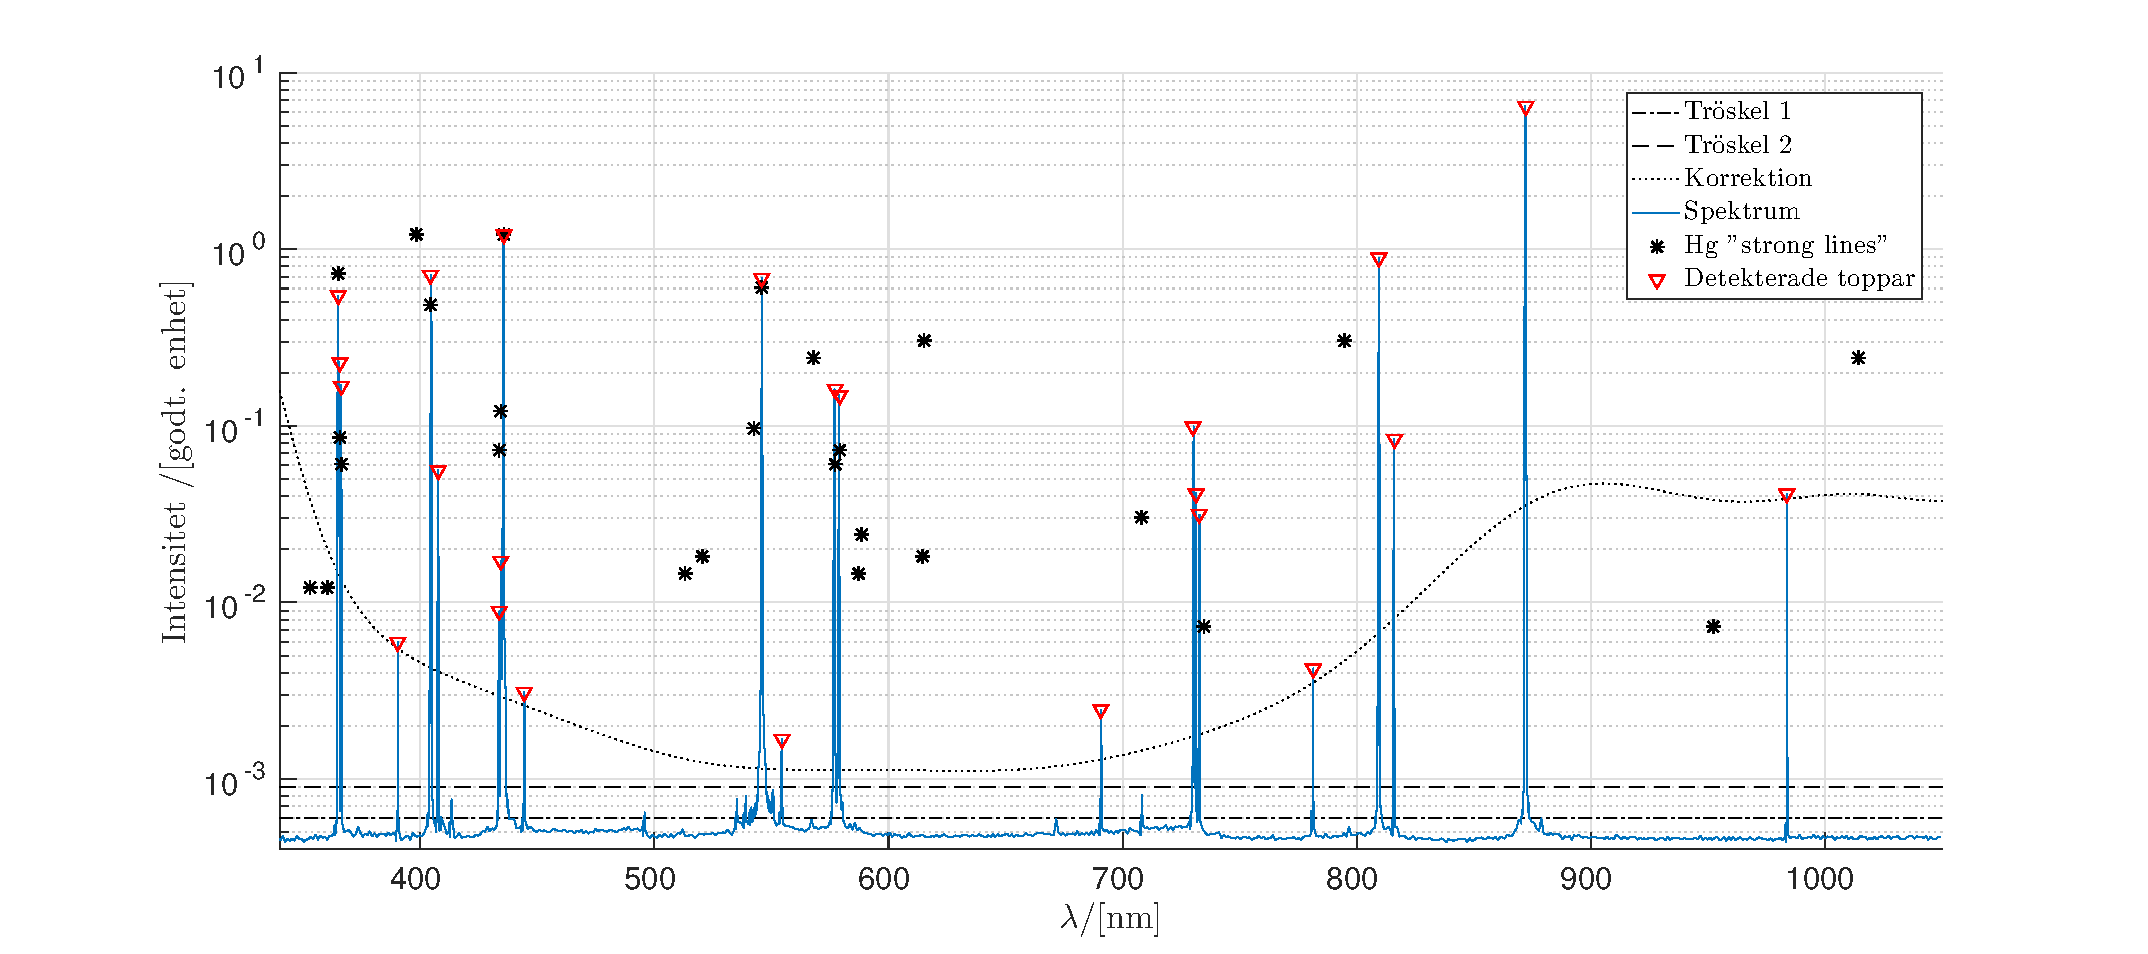
\includegraphics[width=1.2\textwidth]{Hg_spektrum.pdf}
}
\caption{Spektrum uppmätt från kvicksilverlampa tillsammans med
  utmarkerade spektraltoppar enligt NIST\cite{NIST}. De två olika
  typerna av tabellerade data från NIST kallas ''persistent''
  respektive ''strong lines''; skillnaden mellan dessa två tabeller är
  att ''persistent lines'' är de spektrallinjer som syns tydligast
  då det även förekommer orenheter i provet som kan blockera vissa
  övergångar, medan ''strong lines'' är alla starka spektrallinjer som
  förekommer hos ett rent prov.
  Av de två trösklarna som är utritade, styr den första när en en topp
  ska anses stor nog för att det ska vara intressant att minska
  steglängden i våglängd, och den andra tröskeln styr när korrektionen
  ska användas. Korrektionen används bara för de toppar som når över
  den andra tröskeln för att inte den bredare basen på en topp ska
  orsaka att hela toppen ser allt för bred ut. Notera att intensiteten
  är ritad med log-skala, vilket gör att korrektionsfaktorn effektivt
  adderas till toppens höjd varför korrektionen är utritad relativt
  tröskelvärdet och alltså inte motsvarande värdet som ges på
  intensitetsaxeln. 
}
\label{fig:Hg_spektrum} 
\end{sidewaysfigure}




\begin{figure}\centering
\centerline{ %centrerar även större bilder
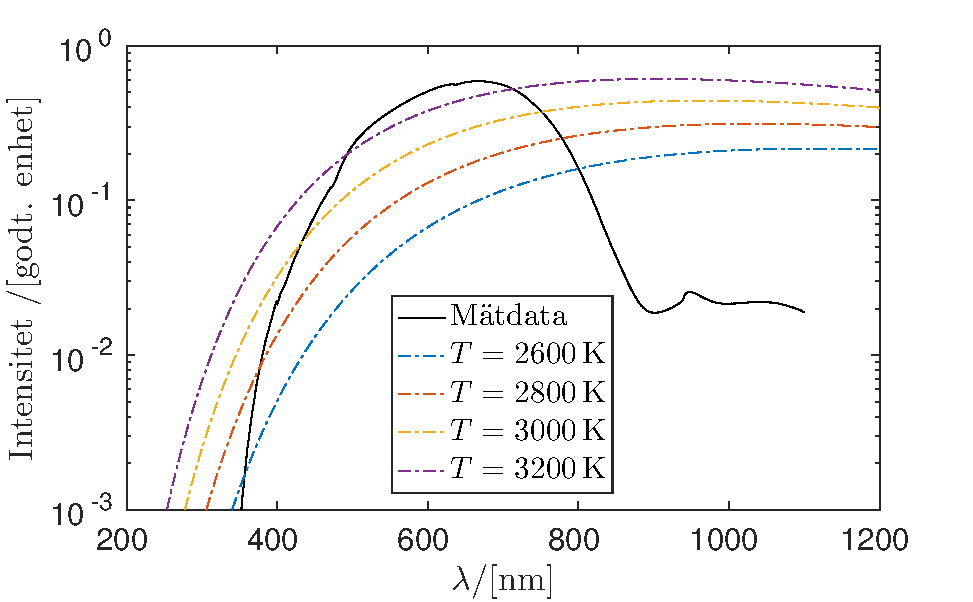
\includegraphics[width=.9\textwidth]{svartkropp.pdf}
}
\caption{Uppmätt spektrum (heldraget) med spektrometern från en
  glödlampa, jämfört med vad Plancks strålningslag ger (normerade
  kurvor). Härifrån syns tydligt att spektrometern har ett ganska
  snävt känslighetsområde där man helst inte bör gå mycket högre än
  till ca 800\,nm våglängd.}
\label{fig:svartkropp}
\end{figure}

\begin{figure}\centering
\centerline{ %centrerar även större bilder
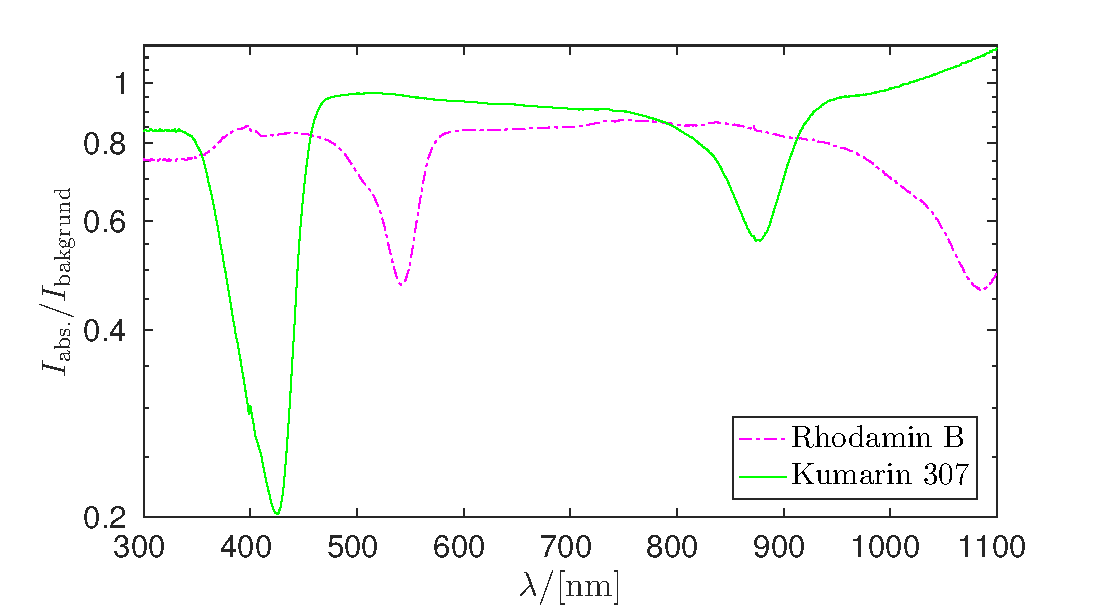
\includegraphics[width=1\textwidth]{absorption.pdf}
}
\caption{Absoprtionsspektrum från Rhodamin B och Kumarin
  307. Absorptionsspektrumen är framtagna som kvoten mellan
  intensiteten som lyste igenom provet mot intensiteten från samma
  ljuskälla utan något prov. Spektrat från glödlampan som användes som
  ljuskälla visas i \figref{fig:svartkropp}. 
}
\label{fig:absorption} 
\end{figure}



 \section{Diskussion}

% I uppgiften med att identifiera energinivåerna i en atom nämndes att
% det är lätt att identifiera de olika energinivåernas inbördes avstånd,
% men att det kan bli svårt att bestämma de absoluta energierna. 

% Det är förvisso sant att det förmodligen inte kommer gå att bestämma
% de absoluta energierna, men även alla inbördes energiskillnader kan
% bli vanskliga att ta fram. Från spektroskopin kommer vi att få ut ett
% antal våglängder som svarar mot en viss energi\-skillnad mellan två
% nivåer. Här måste man nu vara vaksam. Det är ju oftast inte så att
% alla övergångar sker från en viss nivå till den lägsta möjliga nivån;
% vissa övergångar kan ju ske mellan två exciterade tillstånd. Man får
% alltså se om man kan passa ihop flera våglängder svarande mot
% övergångar dels från en exciterad nivå till grundnivån, dels från en
% exciterad nivå till en mellannivå och sen till grundnivån. Detta kan
% bli lite pilligt men inte omöjligt att göra. I övrigt upplevs
% bestämmadet av energinivåerna inte så svårt. 

% För undersökningen av absorption i lösning har vi på förhand inte så
% mycket att utgå från. Vi har åtminstone att lösningsmedlet lär påverka
% energinivåerna i molekylen/jonen. Tidigare resultat för olika
% organiska färgämnen påvisar ett frekvensskift av absorptionstoppen
% beroende på hur polärt lösninsmedlet är \cite{Mannekutla2008}, men
% olika lösningmedel kan även starkt påverka absorptionens intensitet
% \cite{Homocianu2011}.
% I övrigt finns det annat som kan påverka absorptionsspektrat som
% exempelvis jonladdning om man undersöker metalljoner i lösning. 

% Andra förväntade resultat för mätningen av laserfärgämnena är som
% nämnts tidigare att de kommer att sakna distinkta toppar och att de
% flourescerar med längre våglängder än det absorberar. 

\subsection{Hg-spektrum}
%Fattas toppar

\subsubsection{Missade toppar?}

\subsection{Absorptionsspektrum}
%Varför breda dalar och inte skarpa spikar?

\subsection{Upptagningen av spektrumen}
%Enpunktskalibrering
%Känslighetsområde








%För att lägga in en referens så ska den skrivas in enligt mönstret i filen referenser.bib
%Använd \cite{} som vanligt för att använda referensen i texten.
%Här är en bra länk om hur man ska göra:
%https://en.wikibooks.org/wiki/LaTeX/Bibliography_Management#biblatex

\newpage
\iflanguage{swedish}{\renewcommand{\refname}{Källförteckning}}{}
\bibliographystyle{ieeetr}
\bibliography{referenser}


%Detta ser till att bilagorna kommer in snyggt i rapporten/förstudien
\clearpage
\appendix
%\setcounter{section}{0}
%\renewcommand{\thesection}{\Alph{section}}
\setcounter{page}{1}
\renewcommand*{\thepage}{A\arabic{page}}
\phantomsection{}
\iflanguage{swedish}{\renewcommand{\appendixname}{Bilagor}}{}
\addcontentsline{toc}{part}{\appendixname}
\iflanguage{swedish}{\renewcommand{\appendixname}{Bilaga}}{}


\section{Intensitetskorrektion}\label{sec:korr}
Som kan ses i \figref{fig:svartkropp} finns en diskrepans mellan
formen på det uppmätta sprektrat och vad Plancks strålningslag
förutspår. Detta leder till att topparnas höjd i
\figref{fig:Hg_spektrum} inte motsvarar deras faktiska
intensitet.\footnotemark{} Detta gör det svårt att jämföra dessa
mätningarna mot andras resultat. För att ändå kunna göra sådana
jämförelser beräknades korrektionsfaktor, $K$, så att
\[
I_\text{verklig}(\lambda) = I_\text{uppmätt}(\lambda) \cdot K(\lambda).
\]
\footnotetext{Den här effekten har däremot ingen påverkan på
  resultatet för absorptionsspektrat, eftersom det som visas i
  \figref{fig:absorption} är kvoten mellan intensiteterna med och utan
  proverna. }

%\subsection{Fotomultiplikatorn känslighet}
Den huvudsakliga orsaken till det branta tappet i uppmätt intensitet
för våglängder högre än ca 750\,nm beror med största sannolikhet på
fotomultiplikatorns känslighetsområden. Eftersom fotomultiplikatorer
bygger på den fotoelektriska effekten kommer det finnas en viss minsta
fotonenergi som krävs för att slå ut en elektron i det första
steget. Det är troligtvis det som orsakar nämnt tapp i
känslighet. Vidare bör även mätningar över denna kritiska våglängd
betraktas med försiktighet. Detta för att den fotoelektriska effekten,
teoretiskt, inte över huvud taget borde fungera för fotoner med för
lång våglängd. 


\subsection{Temperaturkänslighet}
Det räcker inte med att bara säga att man ska korrigera mätningarna
så att de passar till Plancks strålingslag. Man måste dessutom ange
till vilken temperatur av svartkroppsstrålning man ska anpassa. I det
här fallet valdes att anpassa till 3200\,K. 

I allmänhet hade en högre temperatur haft bättre passform till den
uppmätta spektralkurvan. Men eftersom det var en glödlampa så ligger
glödtrådens temperatur definitivt under 3700\,K, som är wolframs
smältpunkt. 

Så 3200\,K valdes lite godtyckligt, men det var den högsta troliga
temperaturern för glödtråden. Dessutom är den exakta temperaturen att
anpassa sin svartkroppsstrålning till inte så viktig. Detta syns i
\figref{fig:svartkropp} där \emph{formen} på kurvorna till de olika
temperaturerna varierar mycket lite mellan 2600--3200\,K. 


\subsection{Polynomanpassning och resultat}
Korrektionen som beräknas fram behöver kunna beräknas för en
godtycklig våglängd i mätintervallet eftersom de exakta våglängderna
som användes skiljer sig mellan mätningarna. Därför valdes att göra en
polynomanpassning som visas i \figref{fig:korrektionsfaktor}. 

I \figref{fig:korrektionsfaktor} visas de rena kvoterna och
anpassningen i logaritmisk skala, vilket är lite missvisande ur ett
numeriskt perspektiv. Det är nämligen mycket svårt att få med alla
detaljer i de områden där kvoten är liten när variationerna i värde
går över flera storleksordnigar. För att hantera detta problem gjordes
polynomanpassningen till den logaritmerade kvoten: 
\[
P_\text{anpassad} (\lambda) 
\approx \log(\frac{I_\text{Planck}}{I_\text{spektrometer}}).
\]
Detta leder alltså till att den faktiska korrektionsfaktorn blir
\[
K(\lambda) = \exp(P_\text{anpassad}(\lambda)),
\]
vilket är vad som visas i \figref{fig:korrektionsfaktor}.

Att göra en polynomanpassning är alltid en avvägning mellan å ena
sidan att få med så mycket detajer av kurvan som möjligt, och å andra
sidan inte få ett överanpassat polynom. Eller med andra ord hur hög
grad på polynomet man ska anpassa med. Överanpassade polynom får
bättre passning till de punkter som används, men kan resultera i en
sort oönskad svängning i ändpunkterna. 

Polynomet som användes i anpassningen i den här rapporten var av
grad~17. Gradtalet på anpassningspolynomet valdes genom att pröva sig
fram tills det såg ut att passa. Man kan dock redan här se antydningar
om överanpassning till höger i \figref{fig:korrektionsfaktor}, men de
ansågs vara så små och i ett intervall av mindre vikt så inget gjordes
åt dem. 

Det slutglitiga resultatet av korrektionen visas i
\figref{fig:anpassad_svartkropp}. Man kan se att den korrigerade datan
föjer Plancks strålningslag mycket väl utom i några enstaka
punkter. Det är dock inte så farligt, eftersom huvudsyftet med
korrektionen var att grovt kunna jämföra intensiteten på de
detekterade topparna med tidigare resultat. 

\begin{figure}\centering
\centerline{ %centrerar även större bilder
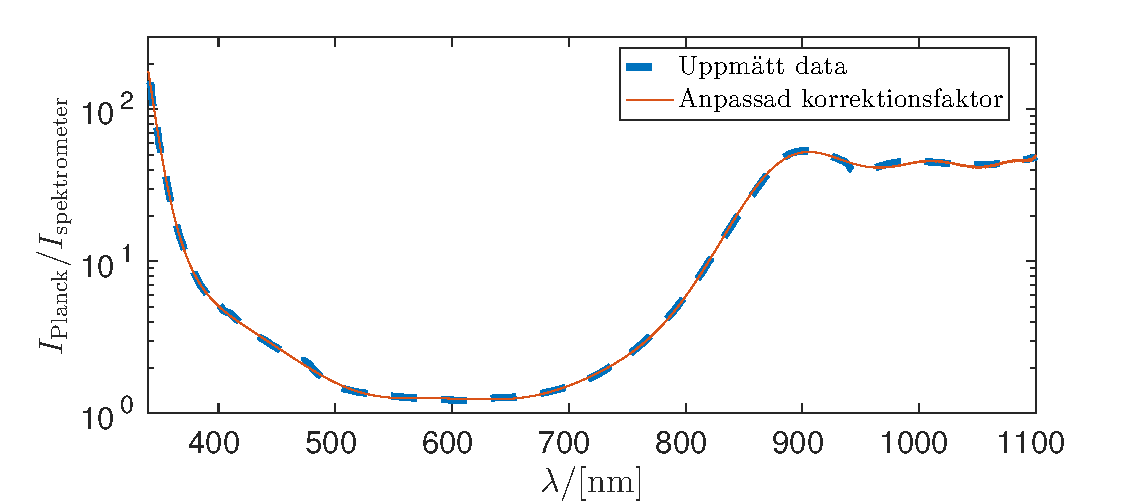
\includegraphics[width=.8\textwidth]{korrektionsfaktor.pdf}
}
\caption{Korrektionsfaktor från kvoten mellan uppmätta spektrumet från
en glödlampa och från Plancks strålningslag. Här visas även
polynomanpassningen som används i \figref{fig:Hg_spektrum}.}
\label{fig:korrektionsfaktor}
\end{figure}

\begin{figure}\centering
\centerline{ %centrerar även större bilder
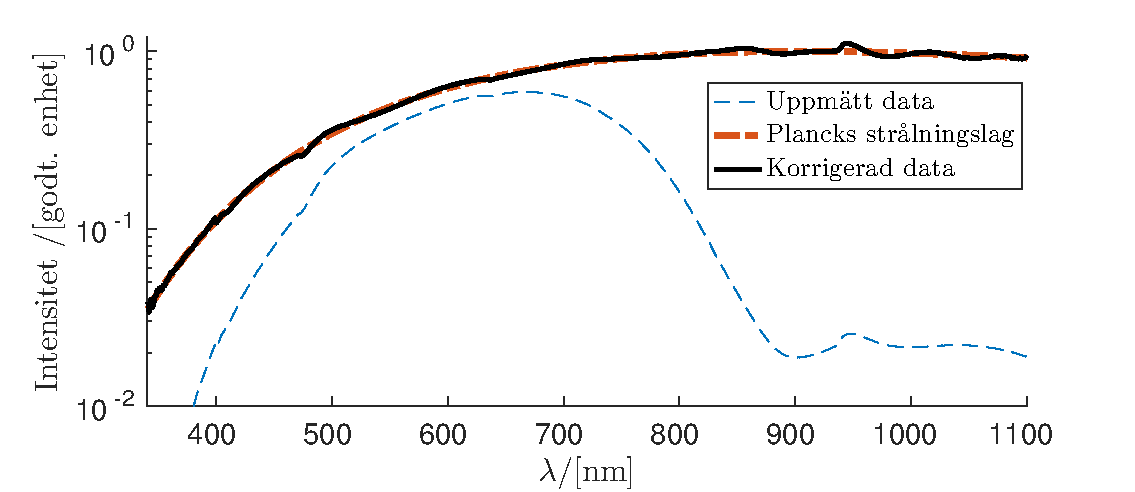
\includegraphics[width=.8\textwidth]{anpassad_svartkropp.pdf}
}
\caption{Jämförelse mellan uppmätt spektrum från en glödlampa och
  Plancks strålnigslag för en svartkropp på 3200\,K tillsammans med
  det korrigerade sprektrat. }
\label{fig:anpassad_svartkropp}
\end{figure}


\section{Kompletterande data}\label{sec:kompl}
Här finns kompletterade, mer noggran presentation av data. I \tabref{tab:Hg_toppar} visas våglängder och motsvarande energier för topparna i \figref{fig:Hg_spektrum}

\begin{table}
\centering
\caption{Våglängder och energier för detekterade toppar (markerade med
  blå trianglar i \figref{fig:Hg_spektrum}) i Hg-spektrumet. } 
\label{tab:Hg_toppar}
\begin{tabular}{|c|c|c|}\hline
$\lambda$/[nm] & $\Delta E$/[eV]  &$\Delta E/[\unit[10^3]{cm^{-1}}$]
\\ \hline
364,94  	& 3,397 	& 27,40 \\ 
365,38  	& 3,393 	& 27,37 \\ 
366,19  	& 3,386 	& 27,31 \\ 
390,50  	& 3,175 	& 25,61 \\ 
404,69  	& 3,064 	& 24,71 \\ 
407,62  	& 3,042 	& 24,53 \\ 
433,75  	& 2,858 	& 23,05 \\ 
434,50  	& 2,853 	& 23,01 \\ 
435,62  	& 2,846 	& 22,96 \\ 
444,44  	& 2,790 	& 22,50 \\ 
546,00  	& 2,271 	& 18,32 \\ 
554,44  	& 2,236 	& 18,04 \\ 
576,94  	& 2,149 	& 17,33 \\ 
578,94  	& 2,142 	& 17,27 \\ 
690,94  	& 1,794 	& 14,47 \\ 
730,31  	& 1,698 	& 13,69 \\ 
731,25  	& 1,696 	& 13,68 \\ 
732,81  	& 1,692 	& 13,65 \\ 
781,44  	& 1,587 	& 12,80 \\ 
809,44  	& 1,532 	& 12,35 \\ 
815,94  	& 1,520 	& 12,26 \\ 
872,00  	& 1,422 	& 11,47 \\ 
983,88  	& 1,260 	& 10,16 \\ 
\hline
\end{tabular}
\end{table}


\end{document}


%% På svenska ska citattecknet vara samma i både början och slut.
%% Använd två apostrofer (två enkelfjongar): ''.

%%För att referera till till tidigare fotnot:
%    \footnotemark[\value{footnote}]

%% Figurer inkluderade som pdf-filer
%\begin{figure}\centering
%\centerline{ %centrerar även större bilder
%\includegraphics[width=1\textwidth]{filnamn.pdf}
%}
%\caption{}
%\label{figuren}
%\end{figure}

%% Figurer inkluderade med xfigs "Combined PDF/LaTeX"
%\begin{figure}\centering
%\input{filnamn.pdf_t}
%\caption{}
%\label{finafiguren}
%\end{figure}

